\chapter{Anforderungen an eine modulare und erweiterbare Bildverarbeitungssoftware}\label{anforderungen}
\addthumb{Anforderungen an das zu entwickelnde Programm}{\huge{\textbf{\thechapter.}}}{white}{haw_rot} 

%\section{Anforderungen an eine modulare und erweiterbare Bildverarbeitungssoftware}\label{einleitung:anforderungen}

Die Software soll grundsätzlich sowohl die Eigenschaften der Modularität, als auch der Erweiterbarkeit besitzen. Die Architektur soll offen für Weiterentwicklungen des Grundsystems sein, damit neue Funktionen leicht eingebaut werden können. Die Variabilität der Software durch Hilfe von Erweiterungen ist wichtig für Lehre und Forschung, um in der Versuchsdurchführung möglichst uneingeschränkt im Bereich der Software zu sein. Bei Bedarf kann eine individueller Ansatz implementiert und in das Programm integriert werden.\\
       
\begin{figure}[htbp]
  \vspace{0.5cm}
  \centering
  \fbox{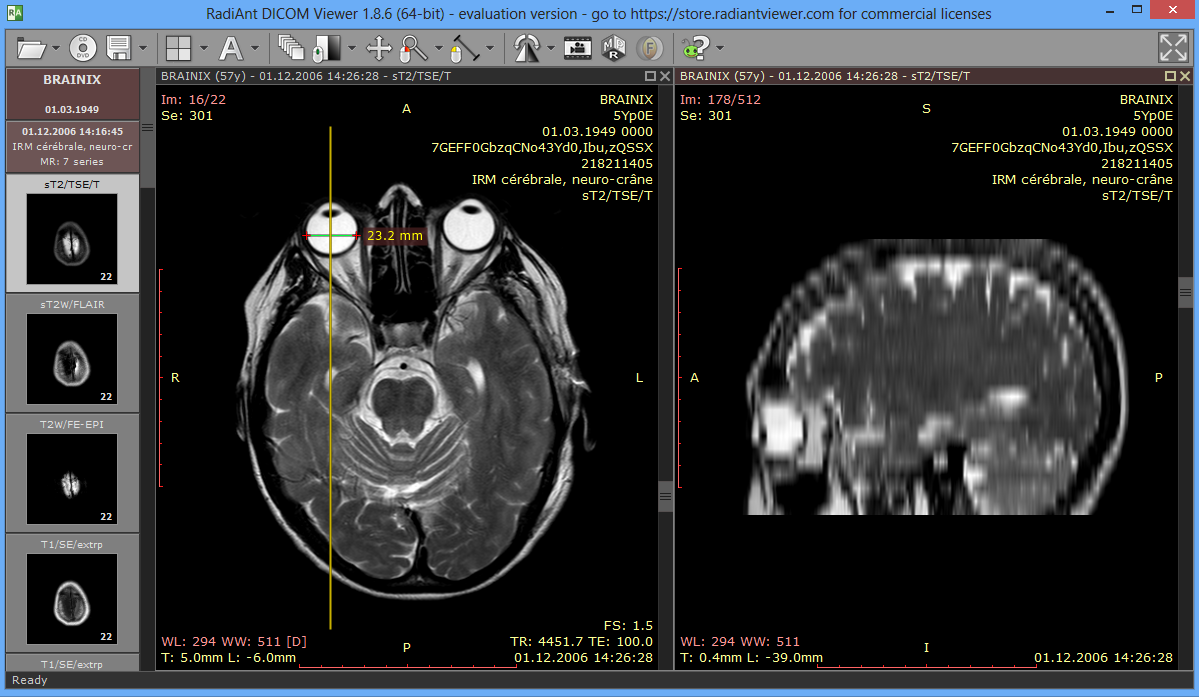
\includegraphics[angle=0,width=9cm]{./img/RadiAnt.png}}
   \caption{RadiAnt - DicomViewer}
  \label{radiant}
  \vspace{0.5cm}
\end{figure}

%\footnotetext{http://www.radiantviewer.com/de/}

% Jetzt eine gleitende Abbildung, die Abbildung wird am oberen 
% Seitenrand positioniert, die Fußnote erhält die Nummer 3
% Der Fußnotenbefehl wird nochmal geschützt

\section{Evaluierung bestehender Software}

Frei verfügbare Software im medizinischen Bereich beschränkt sich oft in den vom Programm vorgegebenen Funktionen und bietet keine Möglichkeit der Erweiterung. Zusätzlich liegt der Fokus auf der Darstellung der Patientenbilder und weniger an den Algorithmen zur Bildverarbeitung. Abbildung \ref{radiant} zeigt den Screenshot des DicomViewers RadiAnt\footnote{http://www.radiantviewer.com/de/}. Die Bilder können einzeln, oder wie auf dem Bild zu sehen, im Bezug zueinander betrachtet werden. Die Werkzeugleiste oben ermöglicht die für DICOM-Bilder typischen Operationen.
Zwar gibt es auf dem Markt auch Open-Source Lösungen mit Schwerpunkt auf Bildverarbeitung, jedoch eigenen sich diese nur bedingt für den Einsatz in der Lehre. Die Programme bieten eine Vielzahl an Funktionen, allerdings benötigt die Entwicklung von Erweiterungen einen erheblichen Zeitaufwand.
 
\begin{figure}[htbp]
  \vspace{0.5cm}
  \centering
  \fbox{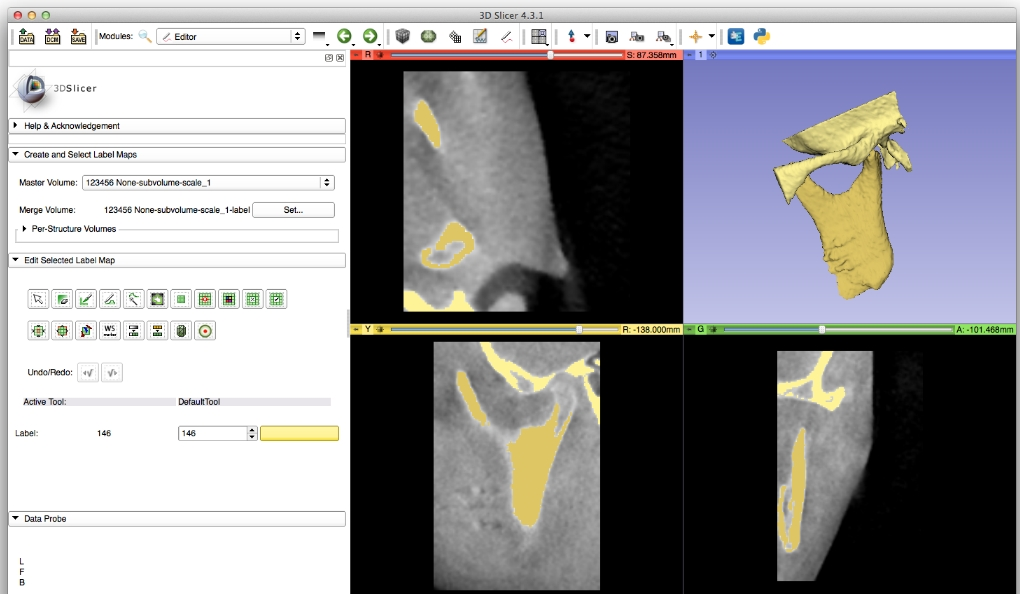
\includegraphics[angle=0,width=9cm]{./img/Screenshot-3DSlicer.png}}
  \floatfoot{Quelle: http://www.linuxlinks.com/portal/content/reviews/Health/Screenshot-3DSlicer.png - abgerufen am 11.01.2014}
  \caption{Screenshot Slicer 3D}
  \label{slicer3d}
  \vspace{0.5cm}
\end{figure}

\section{Slicer 3D}

Slicer 3D\footnote{http://www.slicer.org} (Abbildung \ref{slicer3d}) ist ein umfassendes Werkzeug für die medizinische Bildverarbeitung im zwei- und dreidimensionalen Raum. Die quelloffene Software bietet Möglichkeiten eigene Module zu implementieren. Slicer verwendet als Bibliotheken unter anderem das Insight Toolkit und das Visualization Toolkit\footnote{Insight Toolkit(ITK) und Visualization Toolkit (VTK) sind umfassende Programmbibliotheken zur medizinischen Bildverarbeitung und Visualisierung. Verfasst wurden sie in der Programmiersprache C++}. Das Modul \glqq medizinische Bildverarbeitung\grqq\ baut auf der Programmiersprache Java auf und ist eine weitere Voraussetzung für einen Einsatz im Lehrgebiet. Module in Slicer werden in Python implementiert. Die Studierenden müssten damit eine zusätzliche Sprache lernen.\\

\begin{figure}[htbp]
  \vspace{0.5cm}
  \centering
  \fbox{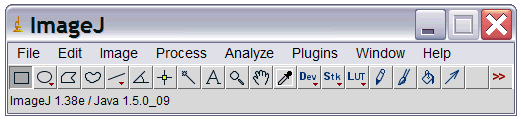
\includegraphics[angle=0,width=9cm]{./img/imagej-window.png}}
  \caption{Die Benutzeroberfläche von ImageJ}
  \floatfoot{ Quelle:  http://rsbweb.nih.gov/ij/features.html - abgerufen am 11.01.2014}
  \label{imagej}
  \vspace{0.5cm}
\end{figure}

\section{ImageJ}

ImageJ ist \glqq State Of The Art\grqq\ im Bereich der Bildverarbeitung in Java\footnote{http://rsbweb.nih.gov/ij/}). Im Grundzustand liefert ImageJ die Standardfunktionen der Bildverarbeitung wie Abbildung \ref{imagej} zeigt. Unter Anderem kann das Bildmaterial analysiert oder mit Filtern bearbeitet werden. ImageJ verarbeitet sowohl Grauwertbilder als auch Farbbilder in den gängigen Formaten wie PNG, JPEG und vielen Anderen. Mit Hilfe der \glqq ImageStacks\grqq\ ist auch eine Bearbeitung im dreidimensionalen Bildraum möglich. Erweiterungen können schnell und zielgerichtet entwickelt werden. Im Modul \glqq Bildverarbeitung\grqq\ der Fakultät Informatik wird ImageJ als Standard zum Bearbeiten der Übungsaufgaben verwendet. Für einen Einsatz im Studiengang Biomedizinische Technik fehlt allerdings die grundlegende Unterstützung von medizinischen Bilddaten im DICOM-Format. Die Funktionalität lässt sich über Plug-ins nachträglich hinzufügen, allerdings fehlt eine Bibliothek die bereits implementierte Algorithmen zur Verfügung stellt, sowie eine Verknüpfung von ImageJ-Klassen wie FloatProcessor oder ByteProcessor in Bildformate der Bibliotheken.

\section{Anforderungen}

Für eine Software die an der Hochschule Landshut für Lehre sowie Forschung im Bereich der medizinischen Bildverarbeitung eingesetzt werden kann ergeben sich folgende Anforderungen:

\begin{itemize}
\item \textbf{Erweiterbarkeit durch den Anwender} \\
	  Anwender sollen die Möglichkeit haben, das Programm mit selbst programmierten Algorithmen zu erweitern. Die eigene Implementierung von Bildverarbeitungsprozessen ist essentiell im Bereich der Lehre.
	  
\item \textbf{Interaktive Benutzereingaben}
	  Aus der Anwendererweiterbarkeit ergibt sich eine weitere Anforderung. Nicht immer können alle Eigenschaften und Werte der Algorithmen während der Implementierung vom Anwender bestimmt werden. Durch die Abhängigkeit von Bilddaten zu Algorithmen muss die Möglichkeit geboten werden, Parameter während der Laufzeit der Anwendung zu bestimmen. Zusätzlich müssen einzelne Bildpunkte interaktiv vom Benutzer ausgewählt und später von Algorithmen benutzt werden können.

\item \textbf{Anwendung der Algorithmen im dreidimensionalen Raum}\\
	  Eine Vielzahl an Bildaufnahmen liegen als dreidimensionaler Datensatz vor. Eine Reihe von Bildern muss folglich zusätzlich zur xy-Ebene auch in z-Richtung zu bearbeiten sein.

\item \textbf{Darstellung aller Ebenen der Bilddaten}\\
	  Ein dreidimensionaler Datensatz macht es möglich, nicht nur die Bilder der xy-Ebene sondern auch die xz- sowie yz-Ebene darzustellen. Es soll möglich sein, in einem Bildsatz einen Punkt auszuwählen und in Darstellungen mit anderer Ebenenansicht der gleichen Daten anzeigen.
	
\item \textbf{Modularer Aufbau} \\
	  Die Software soll auch in den Grundfunktionen erweiterbar sein, die bei Auslieferung des Programms sofort zur Verfügung stehen (Skalierung, Rotation, etc.). Anders als die von Benutzern erstellten Plug-ins, die abhängig vom Anwender sind, muss eine Möglichkeit zur globalen Erweiterung gegeben werden.

\item \textbf{Unterstützung des Dicom-Standards}\\
	  Medizinische Bilddaten besitzen neben den rohen Pixeldaten noch eine Vielzahl zusätzlicher Information wie Patientendaten oder Seriennummern der Aufnahmen und benötigen eine spezielle Verarbeitung. Anders als übliche Grauwertbilder besitzen DICOM-Daten unter Anderem nicht 255 sondern bis zu $2^{16}$ verschiedene Grauwerte.
	  
\item \textbf{Implementierung in der Programmiersprache Java}\\
	  Das Modul zur Bildverarbeitung der Biomedizinischen Technik findet in Java statt. Dadurch wird die Programmiersprache eine Anforderung, da ein Einsatz für die Lehre sonst nur erschwert möglich ist.

\item \textbf{Grundausstattung an medizinischen Bibliotheken}\\
	  Algorithmen in der Bildverarbeitung sind oft komplex und umfangreich. Nicht jeder benötigte Verarbeitungsprozess eignet sich zum selbst implementieren (Sowohl im Lehr- als auch Forschungsbereich). Durch den Einsatz von Bibliotheken wird ein grundlegender Satz an Algorithmen vorgegeben, auf den der Benutzer zurückgreifen und in den Plug-ins verwenden kann.
\end{itemize}

Da in den vorgestellten Anwendungen keine Lösung verfügbar ist, die alle Voraussetzungen erfüllt, soll eine Software entwickelt werden, die für das Labor für medizinische Bildverarbeitung, Algorithmen und Krankenhaus IT die benötigten Anforderungen erfüllt.